% ================================================================================================ %
% Hilfe zum Einstieg in LaTeX
% ================================================================================================ %

% Hier sind ein paar nützliche Links um LaTeX besser lernen zu können und ein paar die es sich zu merken einfach lohnt.

% Ein guter Einstieg ist die Overleaf Dokumentation, diese nimmt dich gut an die Hand.
    % https://de.overleaf.com/learn

% Eine weitere gute Quelle ist "The LaTeX Project", diese bieten einen weiteren gute Dokumentation (auch in De) um hier einen umfassenden Einstig zu finden.
    % https://www.latex-project.org/help/documentation/

% Wenn man schnell LaTeX lernen will empfehle ich die 5 Artikel von Overleaf zum Thesis schreiben
    % https://de.overleaf.com/learn/latex/How_to_Write_a_Thesis_in_LaTeX_(Part_1)%3A_Basic_Structure

% oder die 18 kurze und anschauliche Kapitel von Latex-tutorials.com oder iht Quikstart-Guide
    % https://latex-tutorial.com/tutorials/
    % https://latex-tutorial.com/quick-start/
    
% Auch sinnvoll ist es bei Problemen zu Googeln oder ne KI-Chatbox zu fragen, die meisten können mit LaTeX umgehen und geben aus meiner Erfahrung relativ Sinnvolle antworten

% ======= Resourcen, die Sinnvoll sind %
% Hyperref Anpassungen
    % https://www.namsu.de/Extra/pakete/Hyperref.html
% Biblatex Quide zum einstieg in die Quellen
    % https://de.overleaf.com/learn/latex/Bibliography_management_with_biblatex
% nutzung von Farben in LaTeX (mit xColor)
    % https://latex-tutorial.com/color-latex/
    


\documentclass[             % Basiseinstellungen des Dokuments
12pt,                           % Schriftgröße
a4paper                         % Blattformat
]{report}                       % Art des Textes (Report, Book, Article, ...)
\usepackage[utf8]{inputenc} % Unicode Standart für Sonderzeichen
\usepackage[T1]{fontenc}    % Hinzufügen von mehr Seitenumbrüchen
\usepackage[]{fancyhdr}     % Hinzufügen von mehr Seitenstyles
\pagestyle{fancy}           % Änderung zum "fancy" Seitenstyles
\usepackage[ngerman]{babel} % Deutsches Sprachpaket mit neue Rechtschreibung, d.\,h. (Silbentrennung)
\usepackage[dvipsnames, x11names ]{xcolor} % zusätzliche Farben
\usepackage{multirow}       % Hinzufügen von Tabellen
\usepackage{array}          % Mehr optionen bei Tabellen 
\usepackage{graphicx}       % besseres Hinzufügen und Formatieren von Bildern 
\usepackage[iso, german]{isodate}      % formatieren von Datum, Zeit und Zeitzonen
\usepackage{hyperref}       % Hinzufügen von internen und externen Links
\usepackage{lipsum}         % fügt Text hinzu (Lorem Ipsum)       
  \usepackage[              % fügt Biblatex für vernünftige Quellen ein
    backend=biber,              % Formatierung vom Backend der Quellendokumente
    style=numeric,              % Definiert die Formatierung 
  ]{biblatex}
\usepackage{colortbl}       % Ermöglicht es Tabellen Farbig zu gestalten
\usepackage{movie15}        % Ermöglicht das einbinden von .gif datein durch den befehl
\usepackage{awesomebox}
\usepackage{makecell}       % Ermöglicht linebreaks in Tabellen durch \makecell{} und Überschriften dank \thead{} 

% ================================================================================================ %
% Anpassungen & Befehle
% ================================================================================================ %
% Eine Anmerkung zum Vertikalen Platz


\hypersetup{                % Einstellung von Hyperref
% ======= Dokumentoptionen %
pdftoolbar=true,	% Anzeigen der Acrobat toolbar oder nicht
pdfmenubar=true,	% Anzeigen des Acrobat menu oder nicht
pdftitle={Zusammenfassung Semester 1 Fakultät DM},	% Titel
pdfsubject={lernen},	% Um was geht es
pdfauthor={Nils J. Hack, },	% Autor bzw. Autoren
pdfkeywords={Hochschule Furtwangen, Fakultät Digitale Medien, SoSe24},	% Stichwort1, Stichwort2 ...
pdfcreator={Overleaf},	% Mit welcher Anwendung i.d.R. pdflatex
pdfproducer={Text},	% LaTeX with hyperref
% ======= %
bookmarks=true,	            % erstellt Bookmarks
bookmarksopen=true,        % Anzeigen der Bookmarks beim Öffen des Dokuments
bookmarksnumbered=false,	% Anschnittsnummer anzeigen
% ======= %
    colorlinks=true,            % Farblinks an
    linkcolor=YellowGreen,      % Farbe von internen Verweise
    citecolor=Cerulean,         % Farbe von Zitaten
    urlcolor=RedViolet,         % Farbe zu externen Links
    }

% ============= %
\renewcommand{\footrulewidth}{0.4pt}    % 
% ============= %
\setlength\parindent{0pt}
% ============= %
\setcounter{secnumdepth}{5}
% ============= %

% ======= Quellenbibliotheken hinzufügen %
\addbibresource{Quellen/Medientechnik.bib}


% ======= Formatierungen des Seitenlayouts %
\fancyhead[R]{\rightmark}   % Kopfzeile mit aktueller Section rechts
\fancyhead[L]{\leftmark}    % Kopfzeile mit aktuellem Kapitel oben links
\fancyfoot[R]{\hyperref[TOC]{\textcolor{YellowGreen}{Inhaltsverzeichnis}}}  % fügt unten rechts einen link zum Inhaltsverzeichnis hinzu
\fancyfoot[L]{SoSe24 DM Sem1} % fügt unten links den Text hinzu


% ================================================================================================ %
% Dokument beginnt
% ================================================================================================ %

\begin{document}

% ======= Titelseite anpassen %
\vspace{-5cm}
\title{\vspace{-5cm}\begin{center}
    
\includegraphics[height=100px]{Bilder/HFU_logo.png}
\end{center}\vspace{3cm}Zusammenfassung\\ Semester 1\\ Fakultät DM}
\author{Zusammengefasst von:\\\emph{Nils Hack \& Daniel Georg}}
\date{Im Zeitraum:\\12. Juli 2024 - \today}

% ======= Titelseite %
\maketitle
\setcounter{page}{2} % Setzt Seitenzahl auf 2 weil Deckblatt geskippt wird
\newpage

% ======= Ínhaltsverzeichnis %
\hypersetup{linkcolor=black}    % Setzt die Farbe des Inhaltsverzeichnis zu schwarz, überschreibt das Seitenlayout
\tableofcontents\label{TOC}     % fügt ein label ein um dieses zu Verlinken
\newpage

% ======= Inhalte %             % Durch das hinzufügen von einem "%" die ungewünchten Bereiche ausklammern
\section{Vorwort}
    \subsection{Formattierung}
Unten Rechts am Rand unter \textcolor{YellowGreen}{Inhaltsverzeichnis} ist ein Link der dich wieder nach oben zum Inhaltsverzeichnis bringt.\\~\\
Zudem wird obenlinks das Kapitel und oben rechts das unterkapitel angezeigt um die Orientierung zu verbessern.\\~\\
Im folgenem Dokument werden \\
\textcolor{YellowGreen}{interne Link} in YellowGreen,   \\   
\textcolor{Cerulean}{Quellenverlinkungen} in SeaGreen und \\         
\textcolor{RedViolet}{externe Links} in  RedViolet dargesellt.
    \subsection{Zum Inhalt}
Dies hier zuammengestelten Seiten versuchen ein Gesamtbild aller Vorlesungen abzubilden, die im 1. Semester in der noch so genannten Fakultät Digitale Medien beigebrachten Inhalte näher zu bringen. Dies wird wahrscheinlich nicht im vollem Umfang möglich sein und ich bitte dies zu berücksichtigen. Auch werden wir Versuchen hier aktuelle Klausuraufgaben möglichst gut wiederzugeben, jedoch halten wir uns hier an dem gesetzlichen Rahmen und werden diese entsprechend nicht 1:1 veröffentlichen.\\~\\
Im inhaltlichen Fangen wir bei der SPO an, um einen Rahmen zu bieten und um darauf inhaltlich Aufbauen zu können. Wir Orientieren uns nach der Bennenung nach der SPO und entsprechend sind die Kapitel getaltet. Am Ende von jedem Kurs wollen wir noch kurz mögliche Klausuraufgaben erklären und wo es Sinn ergibt auch das Inhaltliche etwas erweitern und evtl. praktische Tipps näher zu bringen.\\~\\
\emph{Nils}
\chapter{AWBL Maier}

\section{SPO}

    Nachdem Studierende das Modul erfolgreich abgeschlossen haben, können sie:
    \begin{itemize}
        \item Wissen / Kenntnisse\\
            Das Mikro- und Makro-Umfeld von Medienbetrieben, und wie sie diese beeinflussen, benennen sowie den Stellenwert der Medienbranche in der Volkswirtschaft und Gesellschaft skizzieren.
            \newline
            Erklären, wie Medienunternehmen aus betriebswirtschaftlicher Sicht grundlegend funktionieren sowie die relevanten regulatorischen Bedingungen für das Medienmanagement kennen.
        \item Verstehen\\
            Verstehen, wie sich Medienbetrieb unterschiedlicher Art finanzieren sowie verstehen, welche Rechtsformen Medienbetriebe haben können.
            \newline
            Verstehen, welche strategischen und operativen Entscheidungen Medienunternehmen treffen müssen sowie welche Managementinstrumente Medienunternehmen benutzen (können).
        \item Anwenden\\
            Darlegen, in welchem volkswirtschaftlichen, politischen und regulatorischen Bezugsrahmen Medienbetriebe agieren. 
            \newline
            Benennen, wie einzelne Medienbetriebe ihren Markt bzw. ihre Branche definieren und wie sie dies in ihren Aktivitäten beeinflusst.
        \newpage
        \item Analyse\\
            Analysieren, wie Angebot und Nachfrage von Mediengütern zusammenspielen und wie dies von Medienbetrieben koordiniert wird sowie Investitionsentscheidungen in Medienbetrieben analysieren.
            \newline
            Analysieren, wie Medienunternehmen organisiert sind sowie welche Auswirkungen regulatorische Bedingungen auf Entscheidungen im Medienmanagement haben.
        \item Synthesis\\
            Allgemeine personalpolitische Maßnahmen auf Medienbetriebe übertragen.
        \item Evaluation\\
            Steuerliche Konsequenzen medienbetrieblicher Entscheidungen grob bewerten.
            \newline
            Medienbetriebliche Entscheidungen aus Sicht des Controllings bewerten.
    \end{itemize}
    
\newpage
\section{Allgemeine BWL}

\notebox{Aufgabe der Betriebswirtschaftslehre ist es, alles wirtschaftliche Handeln, das sich im Betrieb vollzieht, zu beschreiben und zu erklären und schließlich auf Grund der erkannten Regelmäßigkeiten und Gesetzmäßigkeiten des Betriebsprozesses wirtschaftliche Verfahren zur Realisierung praktischer betrieblicher Zielsetzungen zu entwickeln.}


\newpage\section{Unternehmensgründung}
    \subsection{Grundlagen}

\begin{itemize}
    \item Aus welchen Motiven Gründen Menschen Unternehmen?Was zeichnet einen guten Entrepeneur aus?
    \begin{itemize}
        \item Unzufriedenheit mit Unternehmen
        \item Eigenständigkeit / kein Chef
        \item mehr Freiheiten als Angestellte
        \item höheres Gehalt
        \item Sinnhaftigkeit
        \item eigene Idee Umsetzten
        \item Ausnutzung Marktlücke / Nische
        \item  geringe Auslastung in einem Bereich
    \end{itemize}
    \item Was zeichnet einen guten Entrepreneur aus?
    \begin{itemize}
        \item Kritikfähig
        \item Kompetenz
        \item Work-a-holic
        \item Auslagerung von Kompetenzen
        \item hartnäckig
        \item ausdauernd
        \item Einfühlungsvermögen
        \item Begeisterungsfähigkeit
        \item Überzeugungskraft
        \item Im Interesse des Unternehmens handeln
        \item Verbesserungsfähig
        \item Fehler eingestehen
        \item kein Arschloch
        \item fair sein / beurteilen
        \item nicht nachtragend
    \end{itemize}\newpage
    \item Was sind die Vor- und Nachteile einer Unternehmensgründung?
    \begin{itemize}
        \item höheres Risiko
        \item Insolvenzrisiko
        \item Zeitintensiv
        \item hoher Verwaltungsaufwand
        \item mehr Freiheiten
        \item möglicherweise keine Kunden
        \item höheres persönliches Risiko
        \item anfänglich geringe Gewinne (wenn überhaupt) 
    \end{itemize}
    \item Schritte einer Gründung
    \begin{itemize}
        \item Kapital
        \item Idee
        \item Investment falls nötig
        \item Angestellte
        \item Prototyp
        \item Rechtsform
        \item Business Plans
        \item Kundengewinnung
    \end{itemize}
    \item Faktoren
    \begin{itemize}
        \item Schritte
        \item siehe Risiken
    \end{itemize}
    \item Gründe zum Scheitern
    \begin{itemize}
        \item Schlechte Planung
        \item Unerwartete Ereignisse
        \item Verkalkulation
        \item zu hohe Steuervorzahlungen
        \item schlechte Markteinschätzung
        \item zu hohe Kosten
        \item Mentale Probleme
        \item zu schnelles Wachstum
        \item falsche Prognosen
        \item externe Einflüsse (Katastrophen, Kriege, ...) 
    \end{itemize}
\end{itemize}
    \subsection{Unternehmensplan}
    \subsection{Die 9 Schritte zur Selbstständigkeit}
        \subsubsection{Entscheidung für die Selbstständigkeit}
            \paragraph*{Motive für die Existenzgründung}
            \begin{itemize}
                \item Innovation
                \item Anerkennung
                \item Rollenverhalten
                \item Selbstverwirklichung
                \item Unabhängigkeit
                \item Wirtschaftlicher Erfolg
            \end{itemize}

            
            \paragraph*{Eigenschaften eines Gründers}
            \begin{itemize}
                \item Flexibilität
                \item Machbarkeitsüberzeugung
                \item Risikofreudigkeit
                \item Soziale Kompetenz
                \item Entschlussfreudigkeit
                \item Problemorientierung
                \item Wachstumsorientierung
                \item Durchhaltevermögen
                \item Unabhängigkeitsstreben
                \item Leistungsmotiv
            \end{itemize}
            \paragraph*{ Auslöser der Gründungsaktivität „Theory of planned behavior“}
                „Unternehmensgründungen sind kein spontanes Ereignis zu einem zufälligen Zeitpunkt, sondern das Ergebnis von situativen und kulturellen Faktoren.“\newpage
                \begin{center}
                Äußere oder innere Lebensumstände\\+\\
                Positive Bewertung der Selbstständigkeit\\+\\
                Persönliche hohe Handlungsbereitschaft\\=\\
                Wahrscheinlichkeit der Unternehmensgründung \end{center}
        \subsubsection{Zusammenstellung eines Teams}
            \paragraph{Gründe für eine Gründung im Team}~\\
            \begin{itemize}
                \item Ausgleich der vorhandenen Schwächen (Persönlichkeit, Kompetenz, Know-how)
                \item Größere Finanzkraft
                \item Geteiltes finanzielles Risiko 
                \item Gegenseitige Sparringspartner bei Ideen- und Entscheidungsfindung
            \end{itemize}
            \paragraph{Aber...}~\\
            \begin{itemize}
                \item Verlust an Autonomie
                \item Aufteilen der Erlöse auf mehrere Gründer anteilig an Beteiligung
            \end{itemize}
            \notebox{Eine durchdachte Zusammenstellung des Gründerteams ist entscheidend!}
            \paragraph{Merkmale einer guten Teamzusammenstellung}~\\
            \begin{itemize}
                \item Teile eine gemeinsamen Vision
                \item Gemeinsame Motivation
                \item Hohe Teamfähigkeit und gegenseitige Unterstützung
                \item Offene und regelmäßige Kommunikation
                \item Komplmentäre Eigenschaften und stärken
                \item Klare Vereinbarungen über Eigenstumsverhältnisse
                \item Klare Vereinbarungen über Rechte und Pflichten
                \item Klare Aufteilung der Zuständigkeiten
            \end{itemize}

            \paragraph{Eine häufige Aufteilung in einem Start-Up ist}
            \begin{itemize}
                \item Einer übernimmt die Entwicklung/Technische Leistung
                \item der andere übernimmt den Vertrieb / die kaufmännische Leitung
            \end{itemize}
        \subsubsection{Geschäftsidee entwickeln}
        \subsubsection{Geschäftsmodell konzipieren}
        \subsubsection{Businessplan aufstellen}
        \subsubsection{Finanzierung}
        \subsubsection{Unternehmen gründen}
        \subsubsection{Angebot vermarkten}
        \subsubsection{Erfolg hinterfragen}

    
\input{AWBL/2_AWBL_Prüfungsaufgaben}
\chapter{Medientechnik}

\section{SPO}
    \subsection{Audiotechnik}
        \subsubsection{Lernergebnisse:}
        Nachdem Studierende das Modul erfolgreich abgeschlossen haben, können sie:

        \begin{itemize}
            \item Wissen / Kenntnisse\\
                die AV-technischen Voraussetzungen der computerbasierten Medienproduktion kennen und beherrschen
            \item Verstehen\\
                die physikalischen AV-Grundlagen in computerbasierten Medienanwendungen in Beziehung setzen
            \item Anwenden\\
                die erworbenen theoretischen und technischen Kenntnisse auf konkrete Medienanwendungen übertragen
            \item Analyse\\
                Aufgabenstellungen in computerbasierten Medienproduktionen erkennen und analysieren sowie deren Durchführung planen
            \item Synthesis\\
                infache AV-Produktionen zusammen mit computergenerierten Inhalten durchführen.
            \item Evaluation\\
            etwaige Fehler im computerbasierten AV-Produktionsprozess erkennen und korrigieren.\\
            sicher mit AV-Produktionsequipment umgehen
        \end{itemize}
\newpage
\section{Audiotechnik Reusch}

\subsection{Einstig - Wo finden wir Audio}
\begin{itemize}
    \item Radio
    \begin{itemize}
        \item Information 
        \item Musik
    \end{itemize}
    \item Film
    \begin{itemize}
        \item   Dialog
        \item  FK / SFX
        \item  Musik
        \item  Atmo (natürliche Umgebungsgeräusche)
        \item Geräusche / Foley
    \end{itemize}
    \item Kopfhörer
    \begin{itemize}
        \item Noicecanceling
    \end{itemize}
    \item Durchsagen
    \item Warnsignale
    \item Interface Design
    \item Functional Audio Design
    \item VR
    \item Werbung / Jingles
    \item TV
    \item Games
    \item Synchronsprecher / Voice-Over
    \item Live-/ Beschallung
    \item Theaterton
\end{itemize}
\newpage
\subsection{Schallwellen}


    \subsubsection{Frequenz}
                \paragraph{Definition} 
                    Die Frequenz ist in Physik und Technik ein Maß dafür, wie schnell bei einem periodischen Vorgang die Wiederholungen aufeinander folgen, z. B. bei einer fortdauernden Schwingung. Die Frequenz ist der Kehrwert der Periodendauer.\\Die Einheit der Frequenz ist die abgeleitete SI-Einheit mit dem besonderen Namen Hertz (Einheitenzeichen  Hz); $1 Hz = 1 s-1$ („eins pro Sekunde“). \\~\\~\\
    $f=\frac{\Delta N}{\Delta t}$\\
    $Frequenz=\frac{Anzahl~Wiederholungen}{Zeit}$
    \\~\\

    
    \subsubsection{Periodendauer}
        Dauer einer Schwingung in Sekunden, T = 1/f



    \subsubsection{Amplitude}
        T = Perioden, t= Zeit, Amplitude gibt die Lautstärke an


    \subsubsection{Wellenlänge}
    Die Wellenlänge ist der Abstand zwischen den Wellenbergen, Je Höher die Frequenz, desto kürzer die Wellenlänge\\
 $c=\lambda*f$\\

Ab knapp 20 Wiederholungen werden Klänge und Bilder zu einem einzigen Ton bzw. Video.

\begin{table}[h]
\begin{center}
\begin{tabular}{l|l}
\hline
\rowcolor{YellowGreen!50!} \multicolumn{1}{|l|}{Frequenz} & \multicolumn{1}{l|}{Wellenlänge $\lambda$} \\ \hline
16Hz                           & 21,2m                                      \\
20Hz                           & 17m                                        \\
100Hz                          & 3,4m                                       \\
1.000Hz                        & 0,34m                                      \\
10.000Hz                       & 0,034m                                     \\
16.000Hz                       & 0,021m                                     \\
20.000Hz                       & 0,017m                                    
\end{tabular}
\end{center}
\end{table}
\newpage


    \subsubsection{Oktaven}
    Eine Oktave höher Bedeutet eine verdopplung der [[Frequenz]], dies bedeutet aus 125 Hz werden 250 Hz, 500Hz, 1000Hz, 2000Hz, ...
Dies bedeutet das der Abstand für unsere Ohren der Abstand gleich groß zwischen diesen werten ist und um es entsprechend für unsere Ohren darzustellen werden diese alle Logarythmisch aufgetragen. \\
$20~Hz = \frac{1}{20}Sekunde=50ms$


    \subsubsection{Schallausbreitung}
        Der Tonimpuls wird von Molekühl auf Molekühl weitergetragen, wie eine Welle im Wasser.  Ein Molekühl "schubst"/gibt seine Energie an andere weiter. Es schwingt trotzdem nur an seiner Stelle\\~\\
Der Schall ist eine Wellenbewegung, dieser breitet sich vom Ursprung aus in alle Richtungen aus. Stimmen sind Direktionale Töne, vor dem Kopf besser als hinter dem kopf zu hören. \\~\\
Schallgeschwindigkeit ist für alle Frequenzen gleich schnell, es ändert sich ein wenig bei Temperaturen und nach Stoff wo sich der Schall bewegt.
Eisen z.B. 5km / Sekunde

    \paragraph*{Schallausbreitung}~\\
pro m 3ms = pro km 3sek\\
c bei 0°C: 331,5m/s\\
c bei 20°C: 343m/s


    \subsubsection{Schallbeugung}
        Töne mit langer Wellenlänge beugen sich besser um Hindernisse, weil sie aufgrund ihrem Abstand der Wellen besser um Strukturen herumkommen. 


    \subsubsection{Echogrenze}
        50m/s = 1/20tel Sekunde\\
entspricht 20 Impulsen pro Sekunde = 20Hz


    \subsubsection{Residualeffekt}
    \begin{itemize}
        \item Ohr schliesst aus Obertonstruktur auf (fehlenden) Grundton = Psychoakkustik
        \item Oberwellen addieren sich zur Grundwelle auf (Überlagerung von Wellen)
    \end{itemize}


    \subsubsection{Logarithmische Tonwahrnehmung}
        10 Oktaven sind wahrnehmbar.

\input{Medientechnik/Audiotechnik_Reusch/Ohr_Reusch}
\subsection{Mikrofone}
    \subsubsection{Richtcharakteristiken}
Die Richtcharakteristik gibt an, aus welcher Richtung und wie stark bzw. empfindlich ein Mikro auftreffende Schallwellen aufnimmt. Je nachdem welche Richtcharakteristik ein Mikrofon hat, ist es aus bestimmten Richtungen empfindlicher für Schall als andere Mikrofone. Mikrofone unterscheiden sich in diesem Punkt daher gar nicht so viel von dem menschlichen Gehör – auch wir haben unterschiedliche Arten zu hören und Informationen aufzunehmen: Der Schall von vorne wird lauter empfangen als der Schall von hinten (Abschattungseffekte durch Ohrmuschel).\cite{BeyerRichtchar}
\begin{center}
    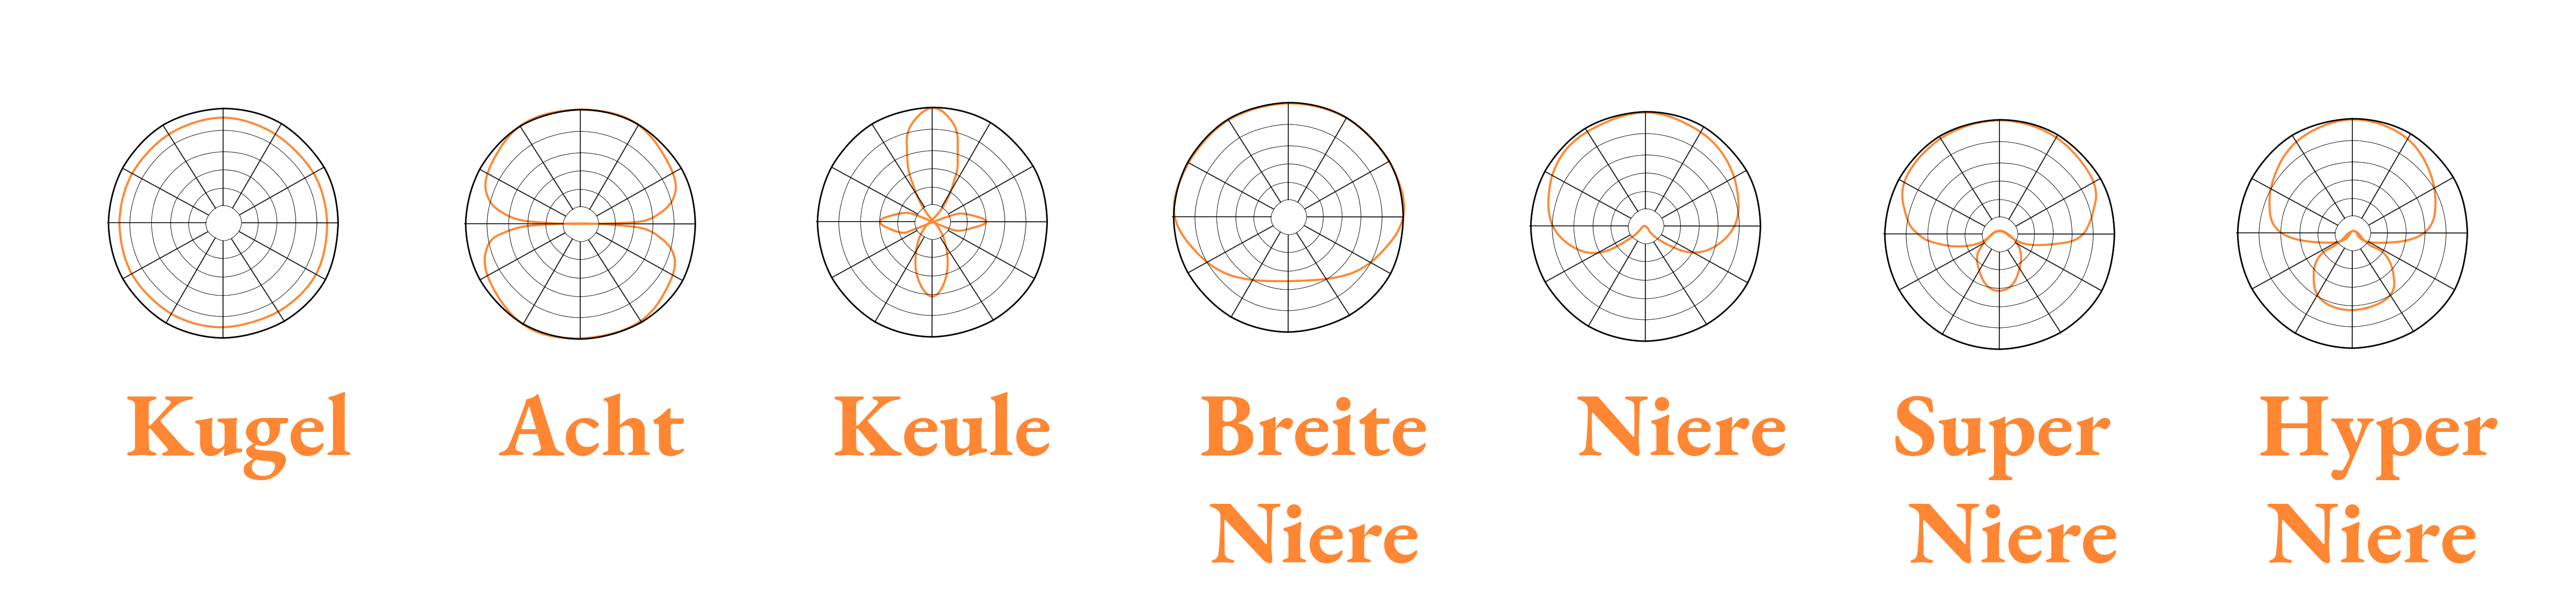
\includegraphics[width=1\textwidth]{Bilder/Medientechnik/Mikrocharakteristik.png}
\end{center}


\subsection{Lokalisation}
Lokalisation ist die Richtungswahrnehmung einer Schallquelle\\~\\
Nicht zu verwechseln mit der Räumlichkeit: Das ist der wahrgenommene Raum, in dem eine Schallquelle zu hören ist.

\subsubsection{Horizontale Lokalisation}
durch interaurale Laufzeitunterschiede und frequenzabhängige Pegelunterschiede. Wir drehen unbewusst den Kopf ständig ein wenig, um genauer zu lokalisieren.\\

\textbf{Lokalisierung auf der Horizontalebene möglich durch:}\\
\paragraph{Interaurale laufzeitdifferenz}~\\
durch 17cm Ohrenabstand max. 0,63 ms. Geringste wahrnehmbare Differenz liegt bei 0,03 ms, entsprechend 3°-5° aus der Mitte, entsprechend 1 cm Laufzeitunterschied.
\paragraph{Pegeldifferenzen}~\\
zwischen linkem und rechtem Ohr: Unterhalb 300Hz keine Unterschiede aufgrund Beugung um den Kopf. Oberhalb gibt es Pegelunterschiede, also Spektraldifferenzen, die zur Ortung führen. Ungenauer als Laufzeitunterschiede!\\~\\
Ohr wertet im Bereich oberhalb 1600 Hz Laufzeit und Pegel aus und ist sehr präzise. Unterhalb von 1600Hz wird vorwiegend die Laufzeit ausgewertet.

\subsubsection{Vertikale Lokalisation}
nur durch durch spektrale Veränderungen, Einfluss der Ohrmuscheln: Richtungsbestimmende (Frequenz)-Bänder nach Blauert:

Und: unser Ohr kann aus den Reflexionen des Raumes ebenfalls auf den Standort der Quelle schliessen.
\input{Medientechnik/Audiotechnik_Reusch/Stereo_reusch}
\subsection{Mikrofonierung}
\notebox{Unter Mikrofonierung oder Mikrofonierungstechnik versteht man die situationsgerechte Auswahl und Aufstellung von geeigneten Mikrofonen zur Aufnahme von Schallquellen. Dabei bestimmen deren Richtcharakteristik und Frequenzgang die Einsatzgebiete. Je nach Aufstellungsort und Mikrofonanordnung sowie Zusammenmischung der Signale wird ein anderer Klang erzielt.\cite{dewiki:Mikrofonierung}}

Im groben sind für uns 3 Arten der Mikrofonierung relevant, die AB-, die XY- und die ORTF-Mikrofonierung. Dabei zu beachten ist das es noch weitere Arten der Aufnahmen gibt, diese 3 sind jedoch typische Vertreter. 

\begin{figure}[h]
    \centering
    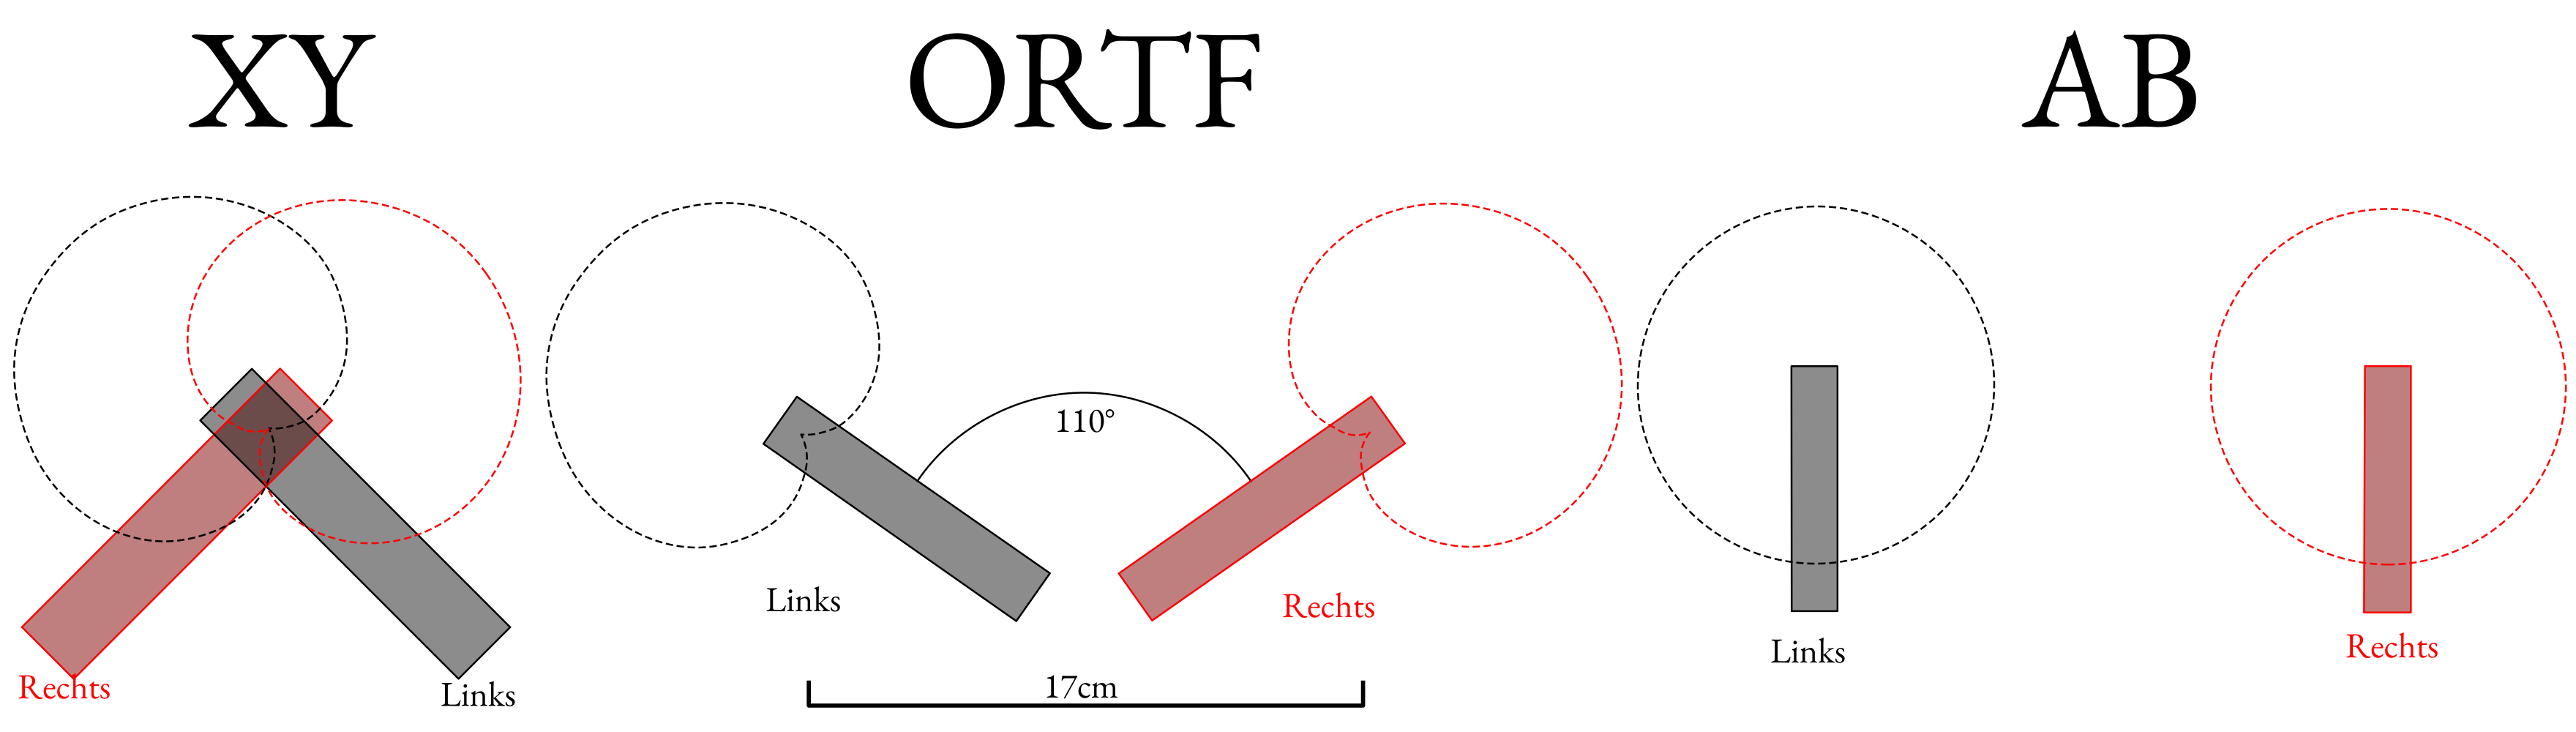
\includegraphics[width=1\linewidth]{Bilder/Medientechnik/Mikrofonierung.png}
    \caption{XY-, ORTF-, und AB-Mikrofonierung}
    \label{fig:Mikrofonierung}
\end{figure}
\newpage

\begin{longtable}
{p{\textwidth/3}p{\textwidth/3}p{\textwidth/3}}
 \label{Mikrofonierung} \\
\toprule
Eigenschaften & Vorteile & Nachteile \\
\midrule
Data 1 & Data 2 & Data 3 \\
Data 4 & Data 5 & Data 6 \\
Data 7 & Data 8 & Data 9 \\
\bottomrule
\end{longtable}

\subsection{Anschlusstechnik}

\subsubsection{Was ist ein balanced Kabel?}
\notebox{Im deutschen heißen balanced Kabel symmetrisch und unbalanced asymetrisch.}
Ein balanced Kabel besteht in unserem Fall meist aus 3 Strängen, 2 für Audioübertragung une einer Erdung (Ground). Die Audioübertragung in den beiden Kabelsträngen wird einmal gespiegelt und daraufhin parallel durch das Kabel geschickt. Wenn eine Störung auftritt wird es in beiden Strängen zeitgleich auftreten und durch die Spiegelung nachträglich wieder zusammengefügt. Da die Störung in die gleiche Richtung auftritt, wird  eine nach der Rückspiegelung ebenfalls gespiegelt. Wenn man nun beide Signale wieder zusammenführt ergibt sich ein Signal wo sich die Störung gegenseitig auslöscht.
\includegraphics[width=1\textwidth]{Bilder/Medientechnik/darstellung Störug.png}\newpage
Bei der Zusammenführung sieht das dann so ungefähr aus, die Spuren werden wieder im Original zusammengelegt (eine zurück gespiegelt) und daraufhin aufaddiert. \\
\includegraphics[width=1\textwidth]{Bilder/Medientechnik/darstellung Störug2.png}

\subsubsection{Beispiele an Anschlusstechnik}
\paragraph{XLR}
~
\begin{figure}[h]
    \centering
    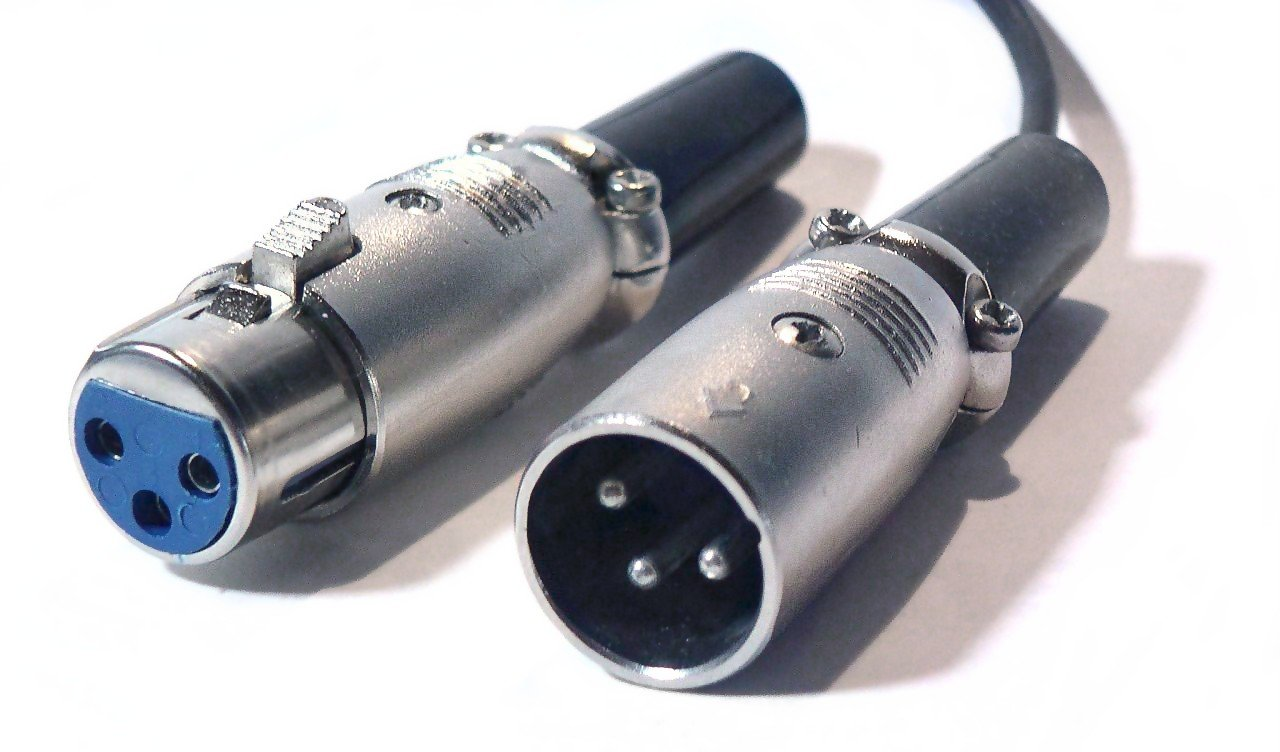
\includegraphics[width=1\textwidth]{Bilder/Medientechnik/Xlr-connectors.jpg}
    \caption{XLR Stecker und Buchse, Bild von Michael Piotrowski\cite{Xlrconne26:online}}
    \label{fig:XLR Stecker \& Buchse}
\end{figure}

links: female, Buchse rechts: male, Stecker\\

XLR steht für \textit{E\textbf{x}ternal \textbf{L}ive \textbf{R}eturn} \cite{AllesXLR:online}, wobei External auch Xcreen/Screen für Masse, Live/Line für Signalübertragungkabel/heiß und Return für Ruckleiterkabel/kalt steht.

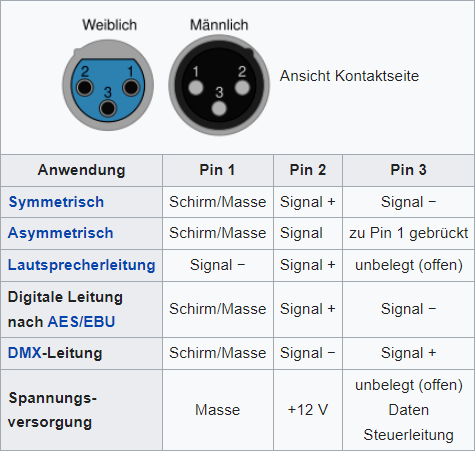
\includegraphics[width=1\textwidth]{Bilder/Medientechnik/XLR-Tabelle.png} \cite{dewiki:241460075}
diese Tabelle zeigt die verschiedenen Konfigurationen eines 3-Poligen-XLR-Kabeln. Diese werden meist im Audiobereich verwendet. Es gibt jedoch auch XLR-Kabel mit bis zu 10-Polen, auch andere Kabel wie DMX (Lichtechnik) nutzen das gleiche Format sind jedoch nicht kompatibel.

\paragraph{Klinkenstecker}
Klinkenstecker gibt es in vielen verschieden Bauarten, jedoch ist ihr Aufbau grundlegend gleich. Sie haben verschieden Größen (Durchmesser): 2,5mm 3,5mm 5,23mm 6,35mm und 7,13mm, die jedoch meist für uns relevanten sind \textbf{6,35mm} für den profesionellen Audiobereich und \textbf{3,5mm} meist für den Heimbereich.\\
Im Aufbau unterscheiden diese sich in der Anzahl an Polen, die Bezeichnung dieser hängt auch von der Anzahl ab. T, R und S sind die kürzel für \textbf{T}ip, \textbf{R}ing und \textbf{S}leeve.\\

\begin{longtable}{|p{0.2\textwidth}|p{0.3\textwidth}|p{0.5\textwidth}|}
\hline
\rowcolor{gray!50} Bezeichnung & Abgeleitet von & Verwendung für \\
\hline
\endfirsthead

\hline
Header 1 & Header 2 & Header 3 \\
\hline
\endhead

\hline
\endfoot

\hline
\endlastfoot

TS & Tip + Sleeve & Monostecker \\
\hline
 \vspace{1mm}TRS & Tip + Ring + Sleeve & Stereostecker oder einkanalige sym- metrische Signalübertragung \\
\hline
TRRS & Tip + Ring + Ring + Sleeve & Stecker mit Zusatzkontakt ~~~~(typisch: Mikrofon oder Video) \\
\hline
TRRRS & RTip + Ring + Ring + Ring + Sleeve & Stecker mit Zusatzkontakt ~~~~(typisch: Antischall) \\
\hline

\end{longtable}
\cite{dewiki:245747795}


\begin{figure}[h]
    \centering
    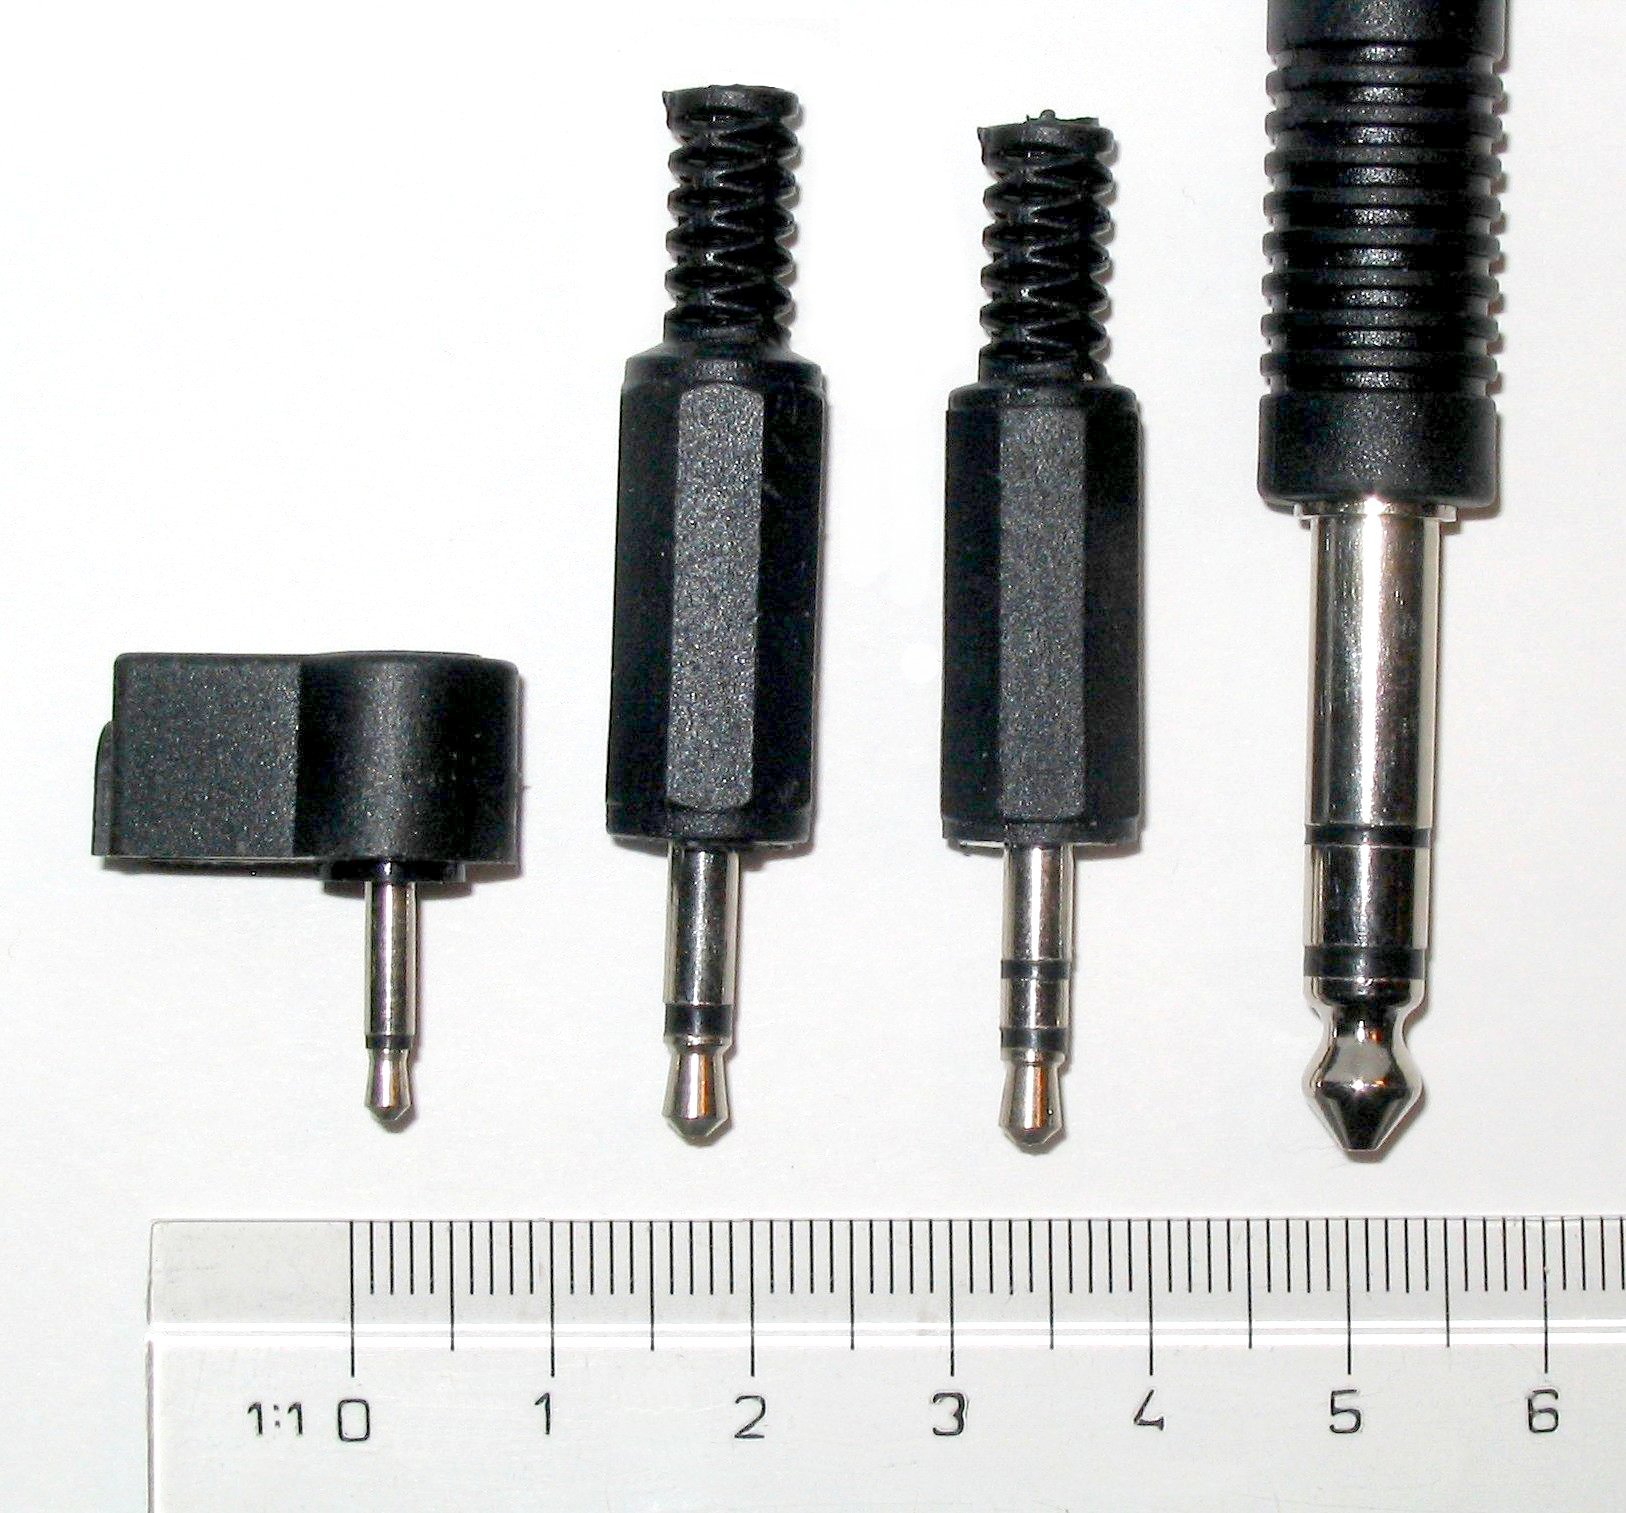
\includegraphics[width=1\textwidth]{Bilder/Medientechnik/Photo-audiojacks.jpg}
    \caption{Beispiele von Klinkensteckern}
    \label{fig:Klinkenstecker}
\end{figure}
\newpage

\paragraph{Chinch}~\\
\begin{figure}[h]
    \centering
    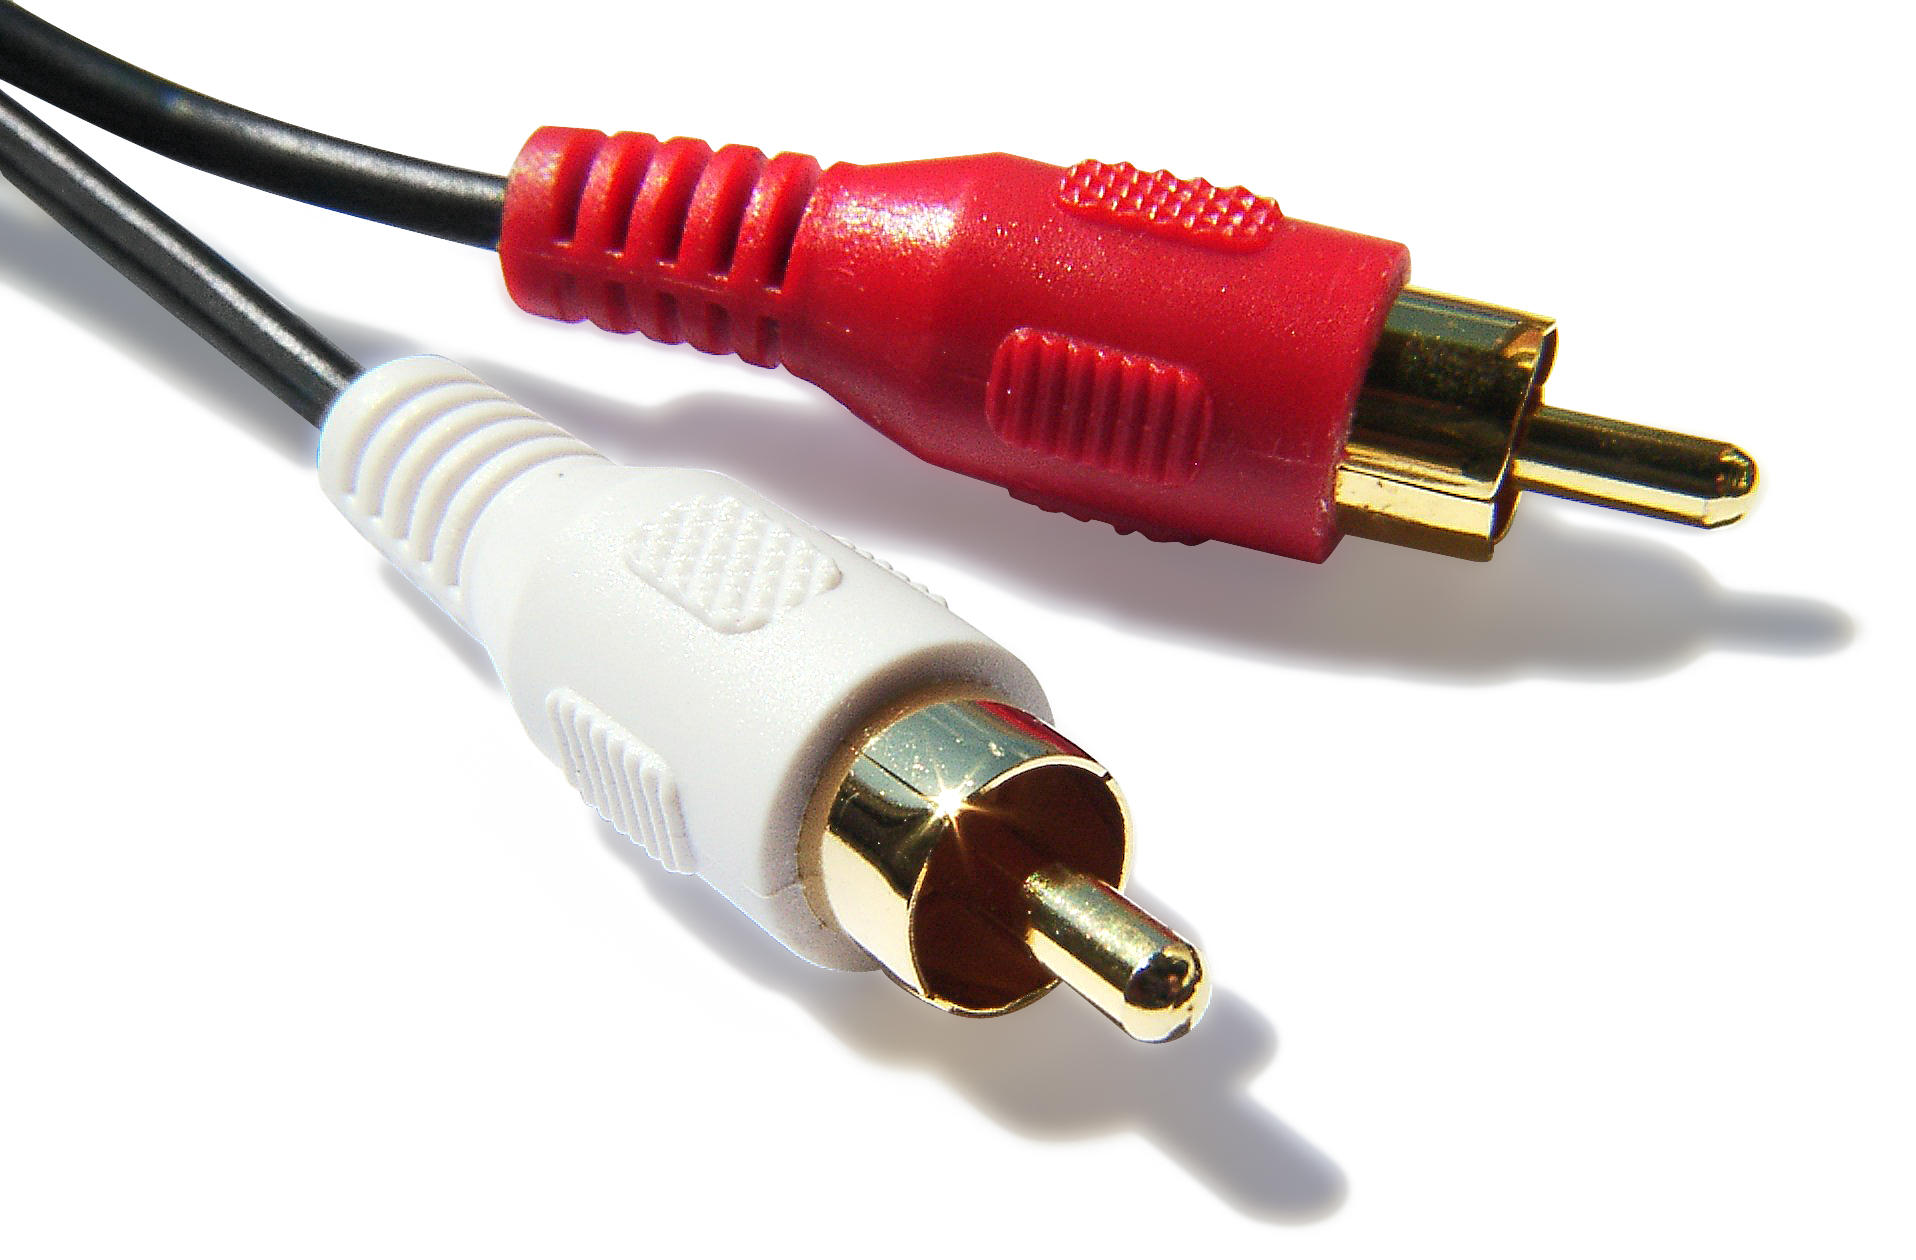
\includegraphics[width=0.5\textwidth]{Bilder/Cinch-Stecker.jpg}
    \caption{Chinch-Stecker: Foto von Wollschaf \cite{wiki:Wollschaf}}
    \label{fig:Chinch}
\end{figure}
~\\
Ein Chinch-Stecker ist ein Audiostecker der oft in Heimberiech für Lautpsrtecher und Anlagen verwendet wird. \cite{dewiki:Chinch}



\paragraph{Multicore-Kabel}
\begin{figure}[h]
    \centering
    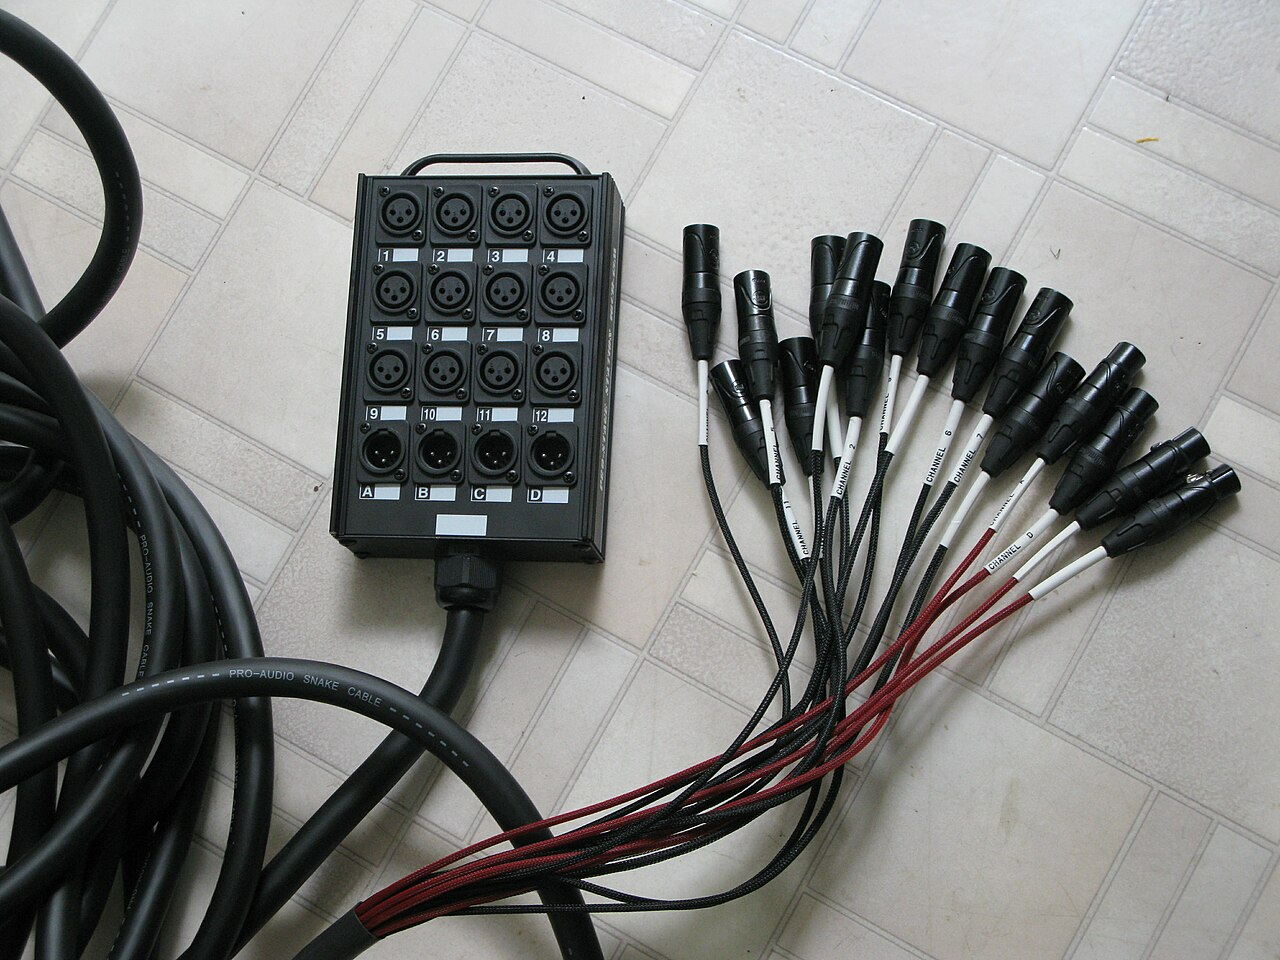
\includegraphics[width=0.5\textwidth]{Bilder/Medientechnik/Audio_multicore_cable_with_XLR_connectors_and_stage_box.JPG}
    \caption{Multicore Kabel: Bild von VK1LW \cite{wiki:VK1LW}}
    \label{fig:Multicore}
\end{figure}~\\
Ein Multicore Kabel ist ein Kabel, das meist ein Bündel von XLR-Kabeln ist. Diese bestehen typischerweise aus einer Stagebox (links) und einer Kabelpeitsche (rechts). In diesem Fall hat das Multicore 16 Stränge, wovon 4 Talkback, kanäle sind. Diese werden meist verwendet um Ton vom Mischpult zurück zu senden, darüber werden dann zum Beispiel Monitore (eine Art Lautsprecher) angeschlossen. \newpage

\subsection{DAW \& Mischpulte}
\subsection{Aufzeichnung}

In diesem Abschnitt geht es um die Wandlung von analogen zu digitalen Signalen (und umgekehrt). Hierbei werden die Klänge durch eine Sinuskurve dargestellt.
\notebox{Bei der Digitalisierung von Klängen gibt es eine Regel die immer beachten werden muss. Die Abtastrate muss mindesten 2x so hoch sein wie die Originalquelle. Der Mensch hört maximal bis zu 20.000Hz, das bedeutet die Abtastrate muss über 40.000 Hz betragen, also 40.001. Üblich ist jedoch 44.100 (CD) und sonst eigentlich 48.000Hz oder ein vielfaches davon.
Wenn dies nicht geschieht (unterabtastung) entstehen neue Schwingungen die im Orhinal nicht vorhanden waren.} 
\paragraph{A/D Wandlung}~
\begin{figure}[h]
    \centering
    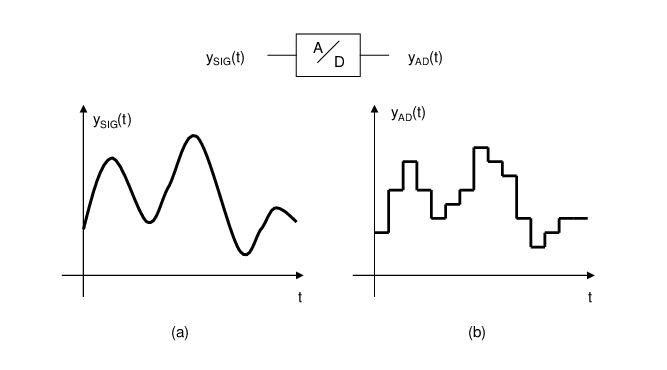
\includegraphics[width=0.8\linewidth]{Bilder/Medientechnik/DA-Wandlung.png}
    \caption{Analog / Digital Wandlung \cite{DA-Wandlung:online}}
    \label{fig:AD-Wandlung}
\end{figure}

Bei der Analog zur Digitalwandlung wird ein Analoges Signal in Form einer Welle aufgenommen und abgetastet. Dann wird in Regelmäßigen Abstanden (z.B. 48.000x pro Sekunde) abgetast. Von der Welle ausgehend wird dann der Wert zum nächsten "Bit" angehoben oder abgesenkt um dann entsprechend eine Spannungskirve zu erzeugen. Im Bild rechts ist dies zu sehen. Jedem dieser Platos wird entsprechend ein Bitwert zugewiesen, die Bitrate (z.B. 16Bit) gibt dann an wie viele von diesen Platos es gibt. 
\cite{DA-Wandlung:online}

\textbf{Eine genauere Erklärung sind in den Unterlagen von Matthias Reusch}


\subsection{Praxisbeispiele}

\subsubsection{RedBull Symphonic}
Eine Herausforderung ein Orchester über Hip-Hop durchzukommen. Hip-Hop ist sehr laut und es erfordert entsprechend viele Mikrophone an den Instrumenten (meist an jedem eines) um die Klassik noch neben dem Hip-Hop zu hören. Ein Problem ist es, dass die Klassische Musik nur bis zu einem gewissen Wert geht und halt nicht höher.
\href{https://youtu.be/2s__lEzWqo4?si=bGhVtFCQNC-s5NzL}{Kool Savas | Red Bull Symphonic - Das Konzert in voller Länge}\\
Abmischung vom Orchester und zusammenarbeit mit \href{https://de.linkedin.com/in/oliver-voges-ab151672}{Olli Voges} (Casper, Cool Savage, Dragonforce, ...)

\subsubsection{Joo Kraus}
\href{https://youtu.be/hrD4D0ShFBY?si=8nK3cuIGO_KtiYv7}{JOO KRAUS / OMAR SOSA / CHAMBER ORCHESTRA ARCATA - Light In The Sky - Live 2017} 

\subsubsection{Sould Diamonds}
\href{https://youtu.be/EeIQMoYi3gU?si=_4K6PZCx4HAfOsjd}{Soul Diamonds - Night in Tunisia}

\subsubsection{Iron Maiden}
Betreut in München, Systemarbeit aka Leutsprecherarbeit (Ausrichten und Konfigurieren)

\subsubsection{Gast}
Herr Reusch mischt auch für die Band seines Sohnes die Songs ab. \href{https://open.spotify.com/intl-de/track/65qo8OLrleFH5bUOsDxRUo?si=49a2ccd60e154820}{Fallen - Gast (Spotify)}

\subsubsection{d\&b Audiotechnik in Ludwigsburg}
In Ludwigsburg testet der Herrsteller \href{https://www.dbaudio.com/global/de/}{d\&b Audiotechnik} seine neue Produkte bei einem Open-Air Festival. \href{https://youtu.be/UBUGswe_Grw?si=p8W6tscHZTbGxhpX}{Hier mal ein Beispiel.} Einige Lautpsrecher von d\&b sind auch bei uns in der Hochschule in Verwendung.
\newpage
\subsubsection{Planungskonzept Saarpolygon}
Im Saarland ist gerade eine Open-Air Bühne in Planung und Herr Reusch versucht dort die lautsprecheraufstellung optimal zu planen. Dies ist bei dem Objekt des \href{www.Opernfestspiele-saarpolygon.de}{Saarpolygons} jedoch aufgrund der einzigartigen Form für eine Bühne sehr anspruchsvoll. So soll das Ochester beispielweise sich in dem Polygon befinden,







\section{Videotechnik Hottong}

\subsection{Lichtphysik \& Lichtgestaltung}
\subsection{Objektive}
\subsection{Menschliche Wahrnehmung von Motion-Pictures}
\subsection{Technische Qualität von Bildern}
\subsection{Die Farbmodelle der Bildverarbeitung}
\subsection{Grundlagen der Generierung leuchtender Bilder}
\subsection{Elektronische Bildaufnahmetechniken}

\chapter{Gestaltung}
    \section{SPO}
    Nachdem Studierende das Modul erfolgreich abgeschlossen haben, können sie:
    \begin{itemize}
        \item Wissen / Kenntnisse\\
            Die Grundlagen gestalterischer Fragestellungen beurteilen.
            \newline
            Theorien zur Medienrezeption benennen.
        \item Verstehen\\
            Kreative Prozesse verstehen und selber erste Gestaltarbeiten anfertigen.
            \newline
            Verstehen, wo wir als Rezipienten und als Produzenten auf wissenschaftliche Erkenntnisse aufbauen können.
        \item Anwenden\\
            Erste Konzeptionen entwickeln und mit den Augen eines Gestalters Kreativarbeit beurteilen. \newline
            Medienpsychologische Theorien anwenden.
        \item Analyse\\
            Gestaltungsparameter untersuchen und Produktionsprozesse darstellen.
            \newline
            Medienpsychologische Prozesse analysieren.
    \end{itemize}
    
\newpage
    \section{Mediengestaltung}

\newpage
    \section{Medienpsychologie}

\newpage
\newpage
\chapter{Programmieren}

Dieser Kurs ist nicht für komplette Progameiranfänger ohne großen Zeitaufwand zu bewältigen. Der Eisenbiegler ist eingeborener Informatiker, jedoch leider nicht ein guter Professor. Ich empfehle euch Java unabhängig von seinen Resourcen zu lernen, seine Übungsaufgaben sind jedoch Sinnvoll konzipiert. Es steigen regelmäßig über mehrere Semester mehrere Personen, meist ohne Vorkentnisse, an der Bildverarbeitungsaufgabe aus.\\
% nicht sehr motivierend bro
Wer einen Onlinekurs nebenbei belegen will empfehle ich Kurse von \href{https://open.hpi.de/courses}{openhpi}, dies sind kostenfreie Kurse. Speziell empfehle ich diesen \href{https://open.hpi.de/courses/javaeinstieg2020}{Java Kurs}, als alternative zu diesem gibt es auch noch die  \href{https://open.hpi.de/courses/javaeinstieg-schule2024}{Schülerversion}.

\newpage
\section{SPO}

    Nachdem Studierende das Modul erfolgreich abgeschlossen haben, können sie:
    \begin{itemize}
        \item Wissen / Kenntnisse\\
            Die Sprachelemente einer imperativen Programmiersprache benennen.
        \item Verstehen\\
            Die Bedeutung eines imperativen Computerprogramms erklären.
        \item Anwenden\\
            Mit einer integrierten Entwicklungsumgebung arbeiten.
        \item Analyse\\
            Den Ablauf eines vorgegebenen imperativen Computerprogramms beschreiben.
        \item Synthesis\\
            Zu einer einfachen Aufgabenstellung ein imperatives Computerprogramm selbstständig implementieren.
        \item Evaluation\\
            Unterschiedliche Computerprogramme in Bezug auf ihre Effizienz miteinander vergleichen.
    \end{itemize}
    
\newpage
\subsection{Theorie}\newpage
\subsection{Übungsaufgaben}

\input{Programmieren/Uebungen_Eisenbiegler/A1P_Einführung}
\input{Programmieren/Uebungen_Eisenbiegler/A2P_ImperativeProg}
\input{Programmieren/Uebungen_Eisenbiegler/A3P_ImperativeProg}
\input{Programmieren/Uebungen_Eisenbiegler/A4P_Bildverarbeitung}
\input{Programmieren/Uebungen_Eisenbiegler/A5P_ImperativeProg}
\input{Programmieren/Uebungen_Eisenbiegler/A6P_Rekursion}
\input{Programmieren/Uebungen_Eisenbiegler/A7P_Objekte}
\input{Programmieren/Uebungen_Eisenbiegler/A8P_VerketteteObjekte}
\input{Programmieren/Uebungen_Eisenbiegler/A9P_ExceptionHandle}
\input{Programmieren/Uebungen_Eisenbiegler/A10P_ExceptionsAbst}
\input{Programmieren/Uebungen_Eisenbiegler/A11P_PersonenImKrankenhaus}
\input{Programmieren/Uebungen_Eisenbiegler/A12P_Fensterbestellung}
\chapter{MINT}
    \section{SPO}

    Nachdem Studierende das Modul erfolgreich abgeschlossen haben, können sie:
    \begin{itemize}
        \item Wissen / Kenntnisse\\
            Geometrische und algebraische Fragestellungen präzise mithilfe der adäquaten Fachbegriffe artikulieren. 
            \newline
            Zentrale Grundbegriffe der Optik sicher wiedergeben.
        \item Verstehen\\
            Mathematische Sinnzusammenhänge und Beweiselemente bzw. Herleitungen erkennen verstehen und wiedergeben. 
            \newline
            Mathematische Modelle physikalischer Phänomene (z.B. geometrisch-optisches paraxiales Arbeitsmodell für abbildende Systeme) verstehen.
        \item Anwenden\\
            Techniken der Vektorrechnung und der Matrixalgebra auf geometrische Probleme anwenden. \newline
            Grundgesetze der Strahlenoptik auf einfache Kameraobjektivmodelle bzw. Fragestellungen der Fotografie anwenden.
        \item Analyse\\
            Geometrische Standardprobleme in der Ebene und im Raum analysieren. 
            \newline
            Angemessen ausgewählte physikalische Systeme und Strukturen selbstständig analysieren und beschreiben.
        \newpage
        \item Synthesis\\
            Für Frage- und Problemstellungen aus (Linearer) Algebra und Geometrie unter den bereitgestellten Hilfsmitteln die jeweils adäquaten auswählen. 
            \newline
            Ein geeignetes eingegrenztes, für die Medientechnik relevantes Thema aus Optik oder Akustik im Überblick darstellen.
        \item Evaluation\\
            Verschiedene Verfahren (z.B. zur Bestimmung affiner Transformationen) hinsichtlich Übersichtlichkeit und Aufwand abwägen.
    \end{itemize}
    
\newpage
    \section{Mathe}
    \begin{itemize}
        \item {Grundlegende Kenntnisse}
        \item{Einheitskreis}
    \end{itemize}
    
    \subsection{Einleitung}
    \subsection{Grundlegendes}
    Dieses kleine Kapitel ist nur ein kleiner Einstieg; Wiederholung von mathematischen Bezeichnungen. Es lohnt sich, in das Buch "Mathematik fuer Informatiker" hineinzuschauen.
\newpage
    \subsection{Einstieg und Wiederhohlung}

\subsubsection{$\sin$ und $\cos$ im rechtwinkligem Dreieck}
Der $\sin$ ist das Verhältnis von der Gegenkathete zur Hypothenuse im rechtwinkligem Dreieck.\\~ \\
$\frac{Gegenkathete}{Hypothenuse}=\sin(\alpha)=\cos(\beta)$\\~\\
Der $\cos$ ist das Verhältnis der Ankathete im Vergleich zur Hypothenuse im rechtwinkligem Dreieck

\subsubsection{$\sin$ \& $\cos$ im Kreis}
\paragraph*{$\sin$ am Einheitskreis}~\\
Die Welle ist das Verhältnis des Sinus am Einheitskreis auf eine x-Achse übertragen.
\paragraph*{$\cos$ am Einheitskreis}~\\
Die Welle ist das Verhältnis des Cosinus am Einheitskreis auf eine x-Achse übertragen.\\~\\
\hyperlink{https://upload.wikimedia.org/wikipedia/commons/f/f3/Sinus_und_Cosinus_am_Einheitskreis.gif}{\textcolor{RedViolet}{\textbf{\fcolorbox{red}{white}{Darstellung von $\sin$ und $\cos$ im Einheitskreis}}}}\\
\input{MINT/Mathe_Lasowski/Tabelle_Bogenmaß}
\subsubsection{Additionstheoreme}
\begin{center}
    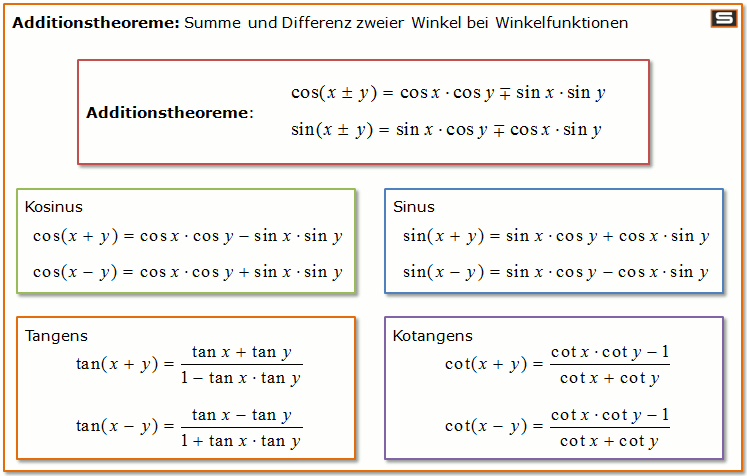
\includegraphics[width=1\textwidth]{MINT/Bilder/Additionstheoreme_Trigonometrie.png}
\end{center}
$sin(x+y)=sin(x)*cos(y)+cos(x)*sin(y)$\\
$sin(30+120)=sin(30)*cos(120)+cos(30)*sin(120)$\\
$=\frac12*-\frac12+\frac{\sqrt3}{2}*\frac{\sqrt3}{2}$\\
$=-\frac14+\frac34=\underline{\frac12}$
\paragraph*{allgemeiner Fall}~\\
\begin{center}
    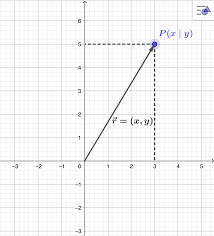
\includegraphics[width=100px]{MINT/Bilder/download 1.png}
\end{center}

\newpage
    \section{Physik}
    \begin{itemize}
        \item{Einleitung}
        \item{Optik abbildender Systeme}
    \end{itemize}

    \subsection{Einleitung}
    Eine physikalische Groesse ist eine quantitativ bestimmbare Eigenschaft von Materie (die Masse eines Steins). Ein Groessenwert ist ein Produkt aus einem Zahlenwert und einer Masseinheit (der Stein wiegt 30kg). 
    \newline
    Eine Groessengleichung ist eine Beziehung zwischen physikalischen Groessen (die Flaeche des Steins setzt sich aus der Breite und der Laenge zusammen).
    \newline
    Das Problem bei Groessengleichung sind oft die unterschiedlichen Zehnerpotenzen. Dafuer gibt es einfache Regeln.
    \subsubsection{Potenzregeln}
        $x^{a} \times x^b = x^{a + b} \iff 10^2 \times 10^3 = 10^{2 + 3} = 10^5$
        \newline
        $\frac{x^a}{x^b} = x^{a - b} \iff \frac{10^4}{10^2} = 10^{4 - 2} = 10^2$
        \newline
        $(x^a)^{^{b}} = x^{a \times b} \iff (10^2)^{^{3}} = 10^{2 \times 3} = 10^6$
        \newline
        $a^n \times b^n = (a \times b)^n \iff 2^2 \times 3^2 = (2 \times 3)^2 = 6^2$
        \newline
        $\frac{a^n}{b^n} = (\frac{a}{b})^n \iff \frac{8^2}{4^2} = (\frac{8}{4})^2 = 2^2$
        \newline

    \subsubsection{SI-Einheiten}
        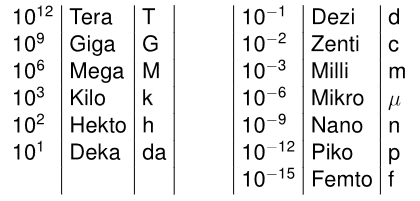
\includegraphics[]{Bilder/MINT/SI.png}
    \newpage
    
\newpage
    \subsection{Optik abbildender Systeme}
    In der geometrischen Optik (Strahlenoptik) wird das Verhalten von Licht vereinfacht modelliert. 
    \newline
    Das Verstaendnis ist wichtig, damit man weiss, wie Bild und Film auf Kamerasensoren treffen. 

    \subsubsection{Optische Systeme}
        Ein Lichtstrahl wird an Grenzflaechen wie bspw. Glas gebrochen. Dadurch entsteht eine Richtungsaenderung. Es gibt mehrere Faelle, aber fuer diesen Kurs wird nur ein Fall betrachtet: Die Strahlen treffen achsennah und parallel auf die Linse ein. Dies nennt man "paraxiale Strahlen". 
        \newline
        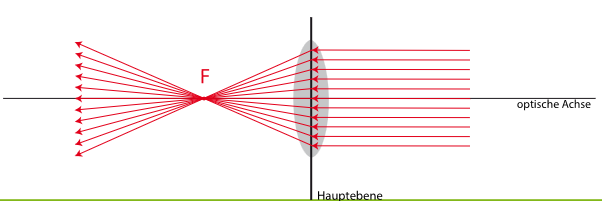
\includegraphics[width=350px]{Bilder/MINT/Paraxiale_Strahlen.png}
        \newline
        In diesem Beispiel treffen die Strahlen von rechts auf die Linse (grau) ein. Die Linse wird auch Hauptebene H genannt. Da Licht bei Glas gebrochen wird, streuen diese auf den bestimmten Punkt F zu, auf dem sie sich alle schneiden. Dieser Punkt F bestimmt, wo die Abbildung scharf ist (Fokus).
        \newline
        \textbf{Wichtig:} Nur, wenn die Strahlen von rechts eintreffen, heisst der Fokus F. Kommen sie links, ist der Fokus F'.
        \newline \newline
        Es gibt auch den Brennpunkt f - dies ist der Abstand des Fokus F von der Hauptebene H.

    \subsubsection{Abbildungsgesetze}
        Generell geht man von drei Faellen aus, was mit einem Lichtstrahl passiert. 
        SEITE 32    
\newpage
    Keine Ahnung :(
\newpage
    \input{MINT/2_MINT_Prüfungsaufgaben}
\newpage
\include{Buecherliste/Bücherliste}
% ======= Quellen %     hinzufügen vom Quellendokument

\addcontentsline{toc}{chapter}{Quellen}
\addcontentsline{toc}{section}{Weblinks}
\printbibliography[type=online,title={Weblinks}] % nur online-artikel

\addcontentsline{toc}{section}{Artikel}
\printbibliography[type=article,title={Articles only}]

\end{document}